\documentclass[11pt]{article}

\usepackage{graphicx, epsfig}
\usepackage{amsmath, amssymb, latexsym}
\usepackage[english]{babel}
\usepackage{amssymb}   
%\usepackage{graphicx}
%\usepackage{float} 






% Make a larger page (shrink the margins)
%
\setlength{\textwidth}{6.7in}
\setlength{\textheight}{9.0in}
\setlength{\evensidemargin}{0.0in}
\setlength{\oddsidemargin}{0.0in}
\topmargin -0.5in
\footskip 0.5in



\title{Progress Report}
\author{Eric}
\begin{document}
\maketitle
\medskip

\begin{figure}[h!]
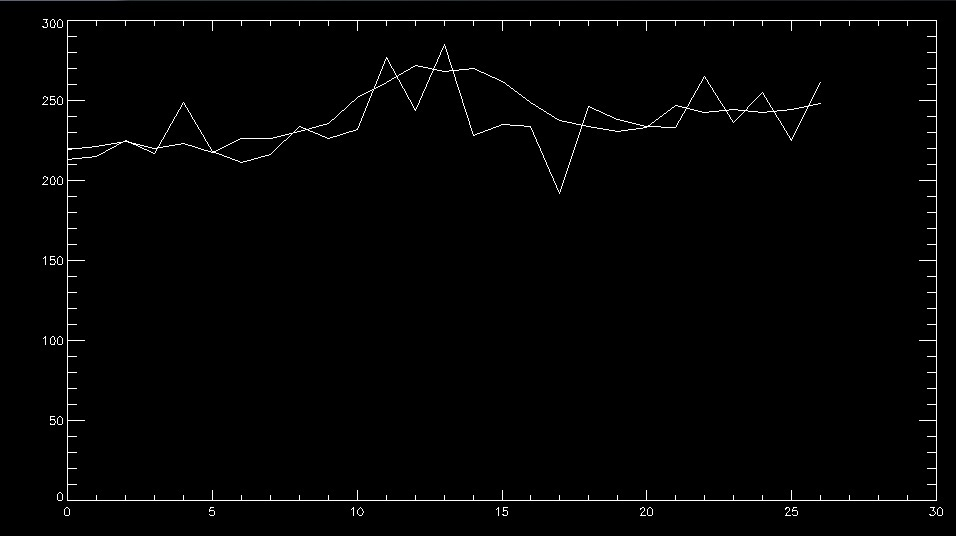
\includegraphics[scale=0.7]{averaging.jpg}
\caption{A comparison of the line profile of the star's peak emission row overlaid with the average counts from the star's entire transit. Clearly the averaging produces a much smoother shape and flattens out most of the background noise}
\end{figure}
\section{Profiling a Star}
\hspace{0.5cm}

The goal of the week was to analyze the shape of the function for a star as it passes overheard. The first part was dedicated to actually finding stars in the keograms (see figure on last weeks weekly report). Since the peak counts for a star are only about two to three times the background noise, I found the best way was to look at smaller areas of the sky at a time. I developed a code that allows you to look at anything from a whole nights worth of data to a single bin, and then plot it. I also looked at the background channels and fitted a polynomial to the background noise, although for the current goals it appears this was an unnecessary step. I used this to subtract out the noise and then calculate the Gaussian shape of the function. I found the row and column in which the maximum counts occurred and used these values to produce a row profile. 

After talking to you I used a method of averaging over the entire stars transit (takes approximately 10 minutes) I was able to produce a plot that has a lot of the noise flattened out. The Gaussfit function performed very well in this regard. I have started making a spreadsheet of A0-A5, the parameters of the stars shape. 





\section{Future Considerations}

I want to compare the functions of several stars from several nights, and tabulate the results. As well, I want to compare the method of fitting a gaussian equation to a function with the background noise subtracted, and see if there is more variation between nights using one method or another. All my code is good to go, so again the biggest chunk of my time in the near future is probably going to be spend finding stars to perform the analysis on.





\end{document}
\end{article}